\chapter{METODOLOGI}

% Ubah konten-konten berikut sesuai dengan isi dari metodologi

\section{Tools Yang Akan Digunakan}

Sistem ini dibuat oleh laptop penulis yang menggunakan \emph{operating system} Arch Linux. Prosesornya sendiri menggunakan Intel Core i5
8265U dan RAM 12 GB. \emph{Graphic Card}-nya adalah NVIDIA GeForce MX 250 2GB. Untuk menggunakan Unreal Engine 5, penulis menggunakan PC
dengan sistem operasi Ubuntu 20.04 dan \emph{Graphic Card} NVIDIA GeFoce GTX 1070 TI. Penulis melakukan remote desktop dengan menggunakan aplikasi
NoMachine.

\subsection{Metamask}
Metamask adalah crypto wallet yang biasanya digunakan untuk keperluan development. Crypto wallet ini
akan sangat membantu dalam proses pengembangan. Terdapat banyak fitur-fitur seperti multi-account yang mempermudah proses pengembangan.

\subsection{Remix IDE}
Remix IDE merupakan IDE yang memudahkan kita untuk proses development, deployment, dan membuat smart contract di Ethereum.

\subsection{Ethereum}
Ethereum adalah \emph{blockchain opensource} dengan fitur smart contract. Fitur smart contract inilah yang akan digunakan untuk 
melakukan sharing data metadata audio.

\subsection{Solidity}
Solidity adalah adalah bahasa tingkat tinggi berbasis objek untuk mengimplementasikan
\emph{smart contract}. Solidity ini dijalankan didalam Ethereum Virtual Machine (EVM).
Kontrak di Solidity mirip dengan class dalam bahasa object-oriented.  Secara umum, Solidity untuk Smart Contract dibuat dengan mengirimkan
Ether ke Smart Contract dan mengirim Ether dari Smart Contract menuju address penerima Ether tersebut.

\subsection{InterPlanetary File System (IPFS )}
Protokol dan peer to
peer network untuk distribusi konten yang cepat, terdistribusi
dan mudah disatukan yang kompatibel untuk semua tipe data
seperti gambar, stream video, database terdistribusi.

\subsection{\emph{web3.storage}}
web3.storage adalah serangkaian API dan layanan yang memudahkan pengembang dan pengguna lain untuk berinteraksi 
dengan data dengan cara yang tidak terikat dengan tempat penyimpanan data sebenarnya secara fisik. Service ini menggunakan data terdesentralisasi dan protokol 
seperti IPFS, Filecoin, dan UCAN yang memungkinkan arsitektur aplikasi dan alur kerja yang dapat diverifikasi, berpusat pada data dan pengguna.

\section{Desain Arsitektur}
Proses ini memberikan perincian pada sistem yang akan dibuat. Berdasarkan dari latar 
belakang masalah dan tujuan dari tugas akhir ini, didapatkan beberapa fungsi yang akan 
diimplementasikan pada sistem dan keseluruhan flow sistem.

\subsection{Arsitektur Sistem}

\begin{figure} [ht] \centering
  % Nama dari file gambar yang diinputkan
  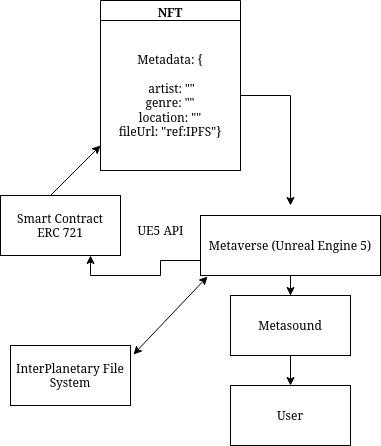
\includegraphics[scale=0.55]{gambar/arsitektur.png}
  % Keterangan gambar yang diinputkan
  \caption{Diagram Arsitektur Sistem}
  % Label referensi dari gambar yang diinputkan
  \label{fig:Architecture}
\end{figure}

\emph{Smart contract} pada arsitektur berguna untuk melakukan operasi-operasi blockchain seperti
memberikan NFT yang berisi metadata dari audio yang sudah disimpan di blockchain sebelumnya.
Untuk file dari audio itu sendiri direferensikan oleh metadata pada NFT tersebut dan akan diambil dari
IPFS menggunakan web3.storage. Metaverse disini diimplementasikan menggunakan Unreal Engine 5 dan menggunakan API
\emph{blockchain} untuk mengeksekusi smart contract. File audio akan diolah oleh metasound dan user akan menerima output audio tersebut.
Untuk deskripsi dari metadata tersebut adalah berupa file JSON dan berikut ini merupakan \emph{interface}-nya

% Contoh input potongan kode dari file
\lstinputlisting[
  language=Python,
  caption={Format data audio.},
  label={lst:formatdataaudio}
]{kode/audioData.json}
Proses perancangan dari arsiktektur sistem yang meliputi IPFS, server, dan blockchain.

\subsection{Proses \emph{generate} NFT dari audio}

Untuk melakukan generate NFT diperlukan proses yang dinamakan Token minting. 
Crypto minting adalah sebuah proses komputasi untuk memvalidasi informasi, membuat blok baru dan merekam informasi tersebut ke dalam blockchain. 
Dalam proses crypto minting biasanya membutuhkan algoritma konsensus Proof-of-Stake.

\begin{figure} [ht] \centering
  % Nama dari file gambar yang diinputkan
  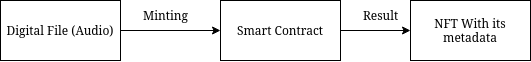
\includegraphics[scale=0.55]{gambar/mintingtoken.png}
  % Keterangan gambar yang diinputkan
  \caption{Diagram Token Minting}
  % Label referensi dari gambar yang diinputkan
  \label{fig:mintingtoken}
\end{figure}

Proof-of-Stake sendiri adalah konsensus yang membantu proses minting seperti bagaimana blok dibuat dan bagaimana data ditambahkan ke blok. Cara kerja crypto minting yaitu koin dicetak (mint) melalui staking di bawah proses Proof-of-Stake. Berbeda halnya dengan Proof-of-Work, Proof-of-Stake tidak memiliki miner. Sebagai gantinya, PoS menggunakan validator. Validator berperan untuk mengamati, juga bertanggung jawab untuk melakukan validasi transaksi dan bekerja untuk menghasilkan blok baru.
Minting adalah proses yang cukup mudah dan terdesentralisasi. Kemudahan dalam proses  minting ini memungkinkan siapa saja untuk membuat token baru tanpa mengharuskan otoritas pusat untuk melakukannya.
Selain itu, ekosistem crypto juga menyediakan berbagai macam token yang diciptakan dengan proses minting, termasuk token aset kripto dan non-fungible token (NFT). Kedua jenis token tersebut tentunya dapat dibuat di berbagai ekosistem blockchain.

\emph{Listing} diatas merupakan \emph{interface} dari metadata yang ditampung di NFT. Semua nilai dari data JSON tersebut 
memiliki tipe data yang adalah \emph{string}

\section{Implementasi}

Pembuatan implementasi dari fitur dari aplikasi yang sudah ditentukan melalui tahap 
sebelumnya. Tahap ini dilakukan sampai selesai untuk masuk pada tahap validasi. Alokasi 
waktu yang ditentukan menyesuaikan dengan pembuatan fitur yang dikerjakan. Pembuatan 
implementasi diperkirakan kurang lebih 1 bulan. Implementasi ini termasuk baik pembuatan mini-metaverse
menggunakan Unreal Engine 5 sebagai sarana untuk melakukan evaluasi dan testing agar keseluruhan sistem dapat terintegrasi.

\subsection{Pembuatan Smart Contract}
Smart Contract diperlukan untuk membuat perjanjian dengan
berbagai kondisi agar pada blokchain bisa mengatur sendiri tanpa
adanya pihak ketika, disini dibuat beberapa kondisi pada
smart contract dalam bentuk kode. Pembuatan smart contract dapat mengacu pada dokumentasi resmi maupun eksternal.
Namun perlu dilakukan modifikasi untuk menyesuaikan dengan desain sistem yang digunakan pada penelitian
ini.

\section{Jadwal Pelaksanaan}

% Ubah tabel berikut sesuai dengan isi dari rencana kerja
\newcommand{\w}{}
\newcommand{\G}{\cellcolor{gray}}
\begin{table}[h!]
  \captionof{table}{Tabel Jadwal Pelaksanaan}
  \label{tbl:timeline}
  \begin{tabular}{|p{3.5cm}|c|c|c|c|c|c|c|c|c|c|c|c|c|c|c|c|}

    \hline
    \multirow{2}{*}{Kegiatan} & \multicolumn{16}{|c|}{Minggu} \\
    \cline{2-17} &
    1 & 2 & 3 & 4 & 5 & 6 & 7 & 8 & 9 & 10 & 11 & 12 & 13 & 14 & 15 & 16 \\
    \hline

    % Gunakan \G untuk mengisi sel dan \w untuk mengosongkan sel
    Requirement Analysis &
    \G & \G & \w & \w & \w & \w & \w & \w & \w & \w & \w & \w & \w & \w & \w & \w \\
    \hline

    Desain Sistem &
    \w & \w & \G & \G & \w & \w & \w & \w & \w & \w & \w & \w & \w & \w & \w & \w \\
    \hline

    Implementasi &
    \w & \w & \w & \G & \G & \G & \G & \G & \w & \w & \w & \w & \w & \w & \w & \w \\
    \hline

    Integration Testing &
    \w & \w & \w & \w & \w & \w & \w & \w & \G & \G & \w & \w & \w & \w & \w & \w \\
    \hline

    Unit Testing &
    \w & \w & \w & \w & \w & \w & \w & \w & \w & \w & \G & \G & \w & \w & \w & \w \\
    \hline

    Evaluasi penelitian &
    \w & \w & \w & \w & \w & \w & \w & \w & \w & \w & \w & \w & \G & \G & \G & \G \\
    \hline

    Penyusunan buku &
    \w & \w & \w & \w & \w & \w & \G & \G & \G & \G & \G & \G & \G & \G & \G & \G \\
    \hline

  \end{tabular}
\end{table}
